% Original: PDF strana 20, donji slajd.
\slajdid{02-s040}
\begin{frame}[label=02-s040]{Susedstvo preko ivica i između slojeva}
\setlength{\parskip}{0pt}
% element: 02-s040:e01
Kartu sa tri promenljive možemo zamisliti u 3D prostoru kao dve preklopljene karte: jednu za \(C=0\), a drugu za \(C=1\).
\par\vspace{1mm}
\begin{columns}[T,onlytextwidth]
\begin{column}{.30\textwidth}\centering
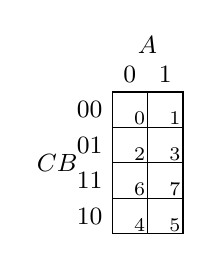
\begin{tikzpicture}[font=\fontsize{9}{10}\selectfont,x=4.5mm,y=4.5mm,baseline=(current bounding box.center)]
\draw (0,0) rectangle (2,4) (1,0)--(1,4);
\foreach \y in {1,2,3}{\draw (0,\y)--(2,\y);}
\node[above] at (1,4.8) {\(A\)};
\node[above] at (.5,4) {0};\node[above] at (1.5,4) {1};
\node[left] at (-.7,2) {\(CB\)};
\foreach \y/\lab in {3.5/00,2.5/01,1.5/11,.5/10}{\node[left] at (0,\y) {\lab};}
\foreach \x/\y/\lab in {1/3/0,2/3/1,1/2/2,2/2/3,1/1/6,2/1/7,1/0/4,2/0/5}{
 \node[anchor=south east,inner sep=.7pt,font=\fontsize{7}{8}\selectfont] at (\x,\y) {\lab};
}
\end{tikzpicture}

\end{column}
\begin{column}{.08\textwidth}\centering\vspace{15mm}\par \(=\)\end{column}
\begin{column}{.58\textwidth}\raggedright
% element: 02-s040:e03
% Zaglavlje C=1 usklađeno je s indeksima 4,5/6,7.
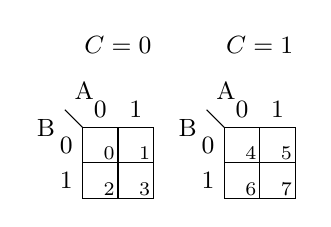
\begin{tikzpicture}[font=\fontsize{9}{10}\selectfont,x=4.5mm,y=4.5mm,baseline=(current bounding box.center)]
\draw (0,0) rectangle (2,2) (1,0)--(1,2) (0,1)--(2,1);
\draw (0,2)--(-.5,2.5) node[above right] {A} node[below left] {B};
\node[above] at (.5,2) {0};\node[above] at (1.5,2) {1};
\node[left] at (0,1.5) {0};\node[left] at (0,.5) {1};
\node[above] at (1,3.8) {\(C=0\)};
\foreach \x/\y/\lab in {1/1/0,2/1/1,1/0/2,2/0/3}{
 \node[anchor=south east,inner sep=1pt,font=\fontsize{7}{8}\selectfont] at (\x,\y) {\lab};
}
\draw (4,0) rectangle (6,2) (5,0)--(5,2) (4,1)--(6,1);
\draw (4,2)--(3.5,2.5) node[above right] {A} node[below left] {B};
\node[above] at (4.5,2) {0};\node[above] at (5.5,2) {1};
\node[left] at (4,1.5) {0};\node[left] at (4,.5) {1};
\node[above] at (5,3.8) {\(C=1\)};
\foreach \x/\y/\lab in {5/1/4,6/1/5,5/0/6,6/0/7}{
 \node[anchor=south east,inner sep=1pt,font=\fontsize{7}{8}\selectfont] at (\x,\y) {\lab};
}
\end{tikzpicture}

\end{column}
\end{columns}
\par\vspace{3mm}
% element: 02-s040:e02
\begin{columns}[T,onlytextwidth]
\begin{column}{.48\textwidth}
\begin{minipage}[c]{.61\linewidth}\raggedright
\Oznaka{Površina 1. reda}\par\vspace{1mm}
U 3D preklapanju susedna su polja \(0\) i \(4\), \(1\) i \(5\), itd. Zato je i grupa \(0,4\) pravilna površina 1. reda.
\end{minipage}\hfill
\begin{minipage}[c]{.36\linewidth}\centering
\begin{tikzpicture}[font=\fontsize{9}{10}\selectfont,x=4mm,y=4mm,baseline=(current bounding box.center)]
\fill[DEcrvena!12] (.06,3.06) rectangle (0.94,4);
\fill[DEcrvena!12] (.06,0) rectangle (0.94,.94);
\draw (0,0) rectangle (2,4) (1,0)--(1,4);
\foreach \y in {1,2,3}{\draw (0,\y)--(2,\y);}
\node[above] at (1,4.8) {\(A\)};
\node[above] at (.5,4) {0};\node[above] at (1.5,4) {1};
\node[left] at (-.7,2) {\(CB\)};
\foreach \y/\lab in {3.5/00,2.5/01,1.5/11,.5/10}{\node[left] at (0,\y) {\lab};}
\foreach \x/\y/\lab in {1/3/0,2/3/1,1/2/2,2/2/3,1/1/6,2/1/7,1/0/4,2/0/5}{
 \node[anchor=south east,inner sep=.7pt,font=\fontsize{7}{8}\selectfont] at (\x,\y) {\lab};
}
\draw[DEcrvena,line width=.8pt,rounded corners=.4mm] (.06,4.2)--(.06,3.06)--(0.94,3.06)--(0.94,4.2);
\draw[DEcrvena,line width=.8pt,rounded corners=.4mm] (.06,-.2)--(.06,.94)--(0.94,.94)--(0.94,-.2);
\end{tikzpicture}

\end{minipage}
\end{column}
\begin{column}{.48\textwidth}
\begin{minipage}[c]{.61\linewidth}\raggedright
\Oznaka{Površina 2. reda}\par\vspace{1mm}
Pravilna površina 2. reda može prekrivati i polja \(0,1,4,5\), preko gornje i donje ivice karte.
\end{minipage}\hfill
\begin{minipage}[c]{.36\linewidth}\centering
\begin{tikzpicture}[font=\fontsize{9}{10}\selectfont,x=4mm,y=4mm,baseline=(current bounding box.center)]
\fill[DEcrvena!12] (.06,3.06) rectangle (1.94,4);
\fill[DEcrvena!12] (.06,0) rectangle (1.94,.94);
\draw (0,0) rectangle (2,4) (1,0)--(1,4);
\foreach \y in {1,2,3}{\draw (0,\y)--(2,\y);}
\node[above] at (1,4.8) {\(A\)};
\node[above] at (.5,4) {0};\node[above] at (1.5,4) {1};
\node[left] at (-.7,2) {\(CB\)};
\foreach \y/\lab in {3.5/00,2.5/01,1.5/11,.5/10}{\node[left] at (0,\y) {\lab};}
\foreach \x/\y/\lab in {1/3/0,2/3/1,1/2/2,2/2/3,1/1/6,2/1/7,1/0/4,2/0/5}{
 \node[anchor=south east,inner sep=.7pt,font=\fontsize{7}{8}\selectfont] at (\x,\y) {\lab};
}
\draw[DEcrvena,line width=.8pt,rounded corners=.4mm] (.06,4.2)--(.06,3.06)--(1.94,3.06)--(1.94,4.2);
\draw[DEcrvena,line width=.8pt,rounded corners=.4mm] (.06,-.2)--(.06,.94)--(1.94,.94)--(1.94,-.2);
\end{tikzpicture}

\end{minipage}
\end{column}
\end{columns}
\end{frame}
